\section{Three-Phase Protocol: Extended Justification}
\label{sec:appendix-phases}

\paragraph{Clutter is the default.}
A robot deployed in a home, warehouse, or lab almost always encounters cluttered scenes---this is the most frequent operating state~\citep{liu2024okrobot, khazatsky2024droid}.

\paragraph{Interaction is the learning signal.}
The fastest-growing paradigm in robot learning is training from human video---a trend spanning representations, policies, and world models.
R3M~\citep{nair2022r3m} and VIP~\citep{ma2023vip} learn visual representations and reward functions from Ego4D~\citep{grauman2022ego4d};
WHIRL~\citep{bahl2022whirl} learns one-shot imitation from unstructured human videos;
MimicPlay~\citep{wang2023mimicplay} learns long-horizon manipulation by watching \textit{human play}---closely mirroring \coolname{}'s interaction phase;
Bharadhwaj~et~al.~\citep{bharadhwaj2023zeroshothuman} demonstrate zero-shot manipulation from passive human videos;
Track2Act~\citep{bharadhwaj2024track2act} predicts point tracks from internet interaction videos;
EgoMimic~\citep{kareer2024egomimic} scales imitation via egocentric video;
EgoDex~\citep{shaw2025egodex} trains dexterous policies from 829 hours of egocentric manipulation;
DROID~\citep{khazatsky2024droid} collects 76K in-the-wild episodes;
and GR-2~\citep{cheang2024gr2} trains VLAs directly from video.
All process human interaction video as input---and perception robustness on this data strongly influences what the robot learns.

\paragraph{Clean reveals recovery.}
Robots rarely encounter tidy scenes, but the clean phase serves as a within-scene control and tests post-manipulation verification.

\paragraph{Why exactly three.}
Two phases would miss the critical interaction state. More than three adds diminishing returns: observe $\to$ act $\to$ verify covers the full manipulation cycle.
Three phases yield three controlled comparisons ($\mathcal{P}_{\text{clu}} \!\to\! \mathcal{P}_{\text{int}}$, $\mathcal{P}_{\text{int}} \!\to\! \mathcal{P}_{\text{cln}}$, $\mathcal{P}_{\text{clu}} \!\to\! \mathcal{P}_{\text{cln}}$) that feed the STR metric.

\paragraph{What each phase reveals per task.}
Table~\ref{tab:phase-per-task-appendix} shows the specific deployment condition each phase tests for each task.

\begin{table}[h]
\centering
\small
\caption{What each phase tests for each task.}
\label{tab:phase-per-task-appendix}
\resizebox{\linewidth}{!}{%
\begin{tabular}{p{1.5cm} p{4cm} p{4cm} p{4cm}}
\toprule
& \textbf{Clutter} & \textbf{Interaction} & \textbf{Clean} \\
\midrule
D1 Depth & Metric accuracy under occlusion & Temporal flicker from hand entry & Accuracy on simpler geometry (control) \\
\addlinespace
D2 Det. & Detection under dense occlusion & Detection during hand occlusion & Reduced occlusion but changed spatial refs \\
\addlinespace
D3 Track & ID maintenance under camera motion & ID survival through hand occlusion & Re-identification after rearrangement \\
\addlinespace
D4 QA & Counting \& attribute QA under clutter & QA when hands occlude objects & Reorganised scene (different answers) \\
\addlinespace
D5 Spatial & Spatial grounding in dense layout & Spatial answers become \textit{wrong} & New arrangement (tests adaptation) \\
\bottomrule
\end{tabular}%
}
\end{table}


\section{ESD Feature Definitions}
\label{sec:appendix-esd-full}

This appendix provides the full mathematical definitions of all 27 ESD features (7 categories) described in Section~\ref{sec:features}.

Given a scene $s$ and phase $p$, let $\mathcal{V}_{s,p} = \{I_t, D_t, M_t, \mathbf{T}_t, F^L_t, F^R_t\}_{t=1}^{T}$ denote the video sequence (RGB, D435 depth, instance mask, SE(3) pose, and T265 left/right fisheye images; the fisheye stream is optional---features default to zero when absent).

\paragraph{Annotation effort.}
Let $\mathcal{K}_{s,p} = \{k_j\}$ be the mask refinement iteration counts:
$f_{\text{iter-mean}} = \frac{1}{|\mathcal{K}|} \sum_j k_j$, \quad $f_{\text{iter-max}} = \max_j k_j$.

\paragraph{Scene complexity.}
Let $\mathcal{O}_t$ be the visible objects in frame $t$, $N_s$ the total annotated objects:
\begin{align}
f_{\text{obj-mean}} &= \frac{1}{T}\textstyle\sum_t |\mathcal{O}_t|, \quad
f_{\text{obj-std}} = \sqrt{\frac{1}{T}\textstyle\sum_t (|\mathcal{O}_t| - f_{\text{obj-mean}})^2} \\
f_{\text{obj-consist}} &= \frac{1}{T}\textstyle\sum_t \mathbb{1}[|\mathcal{O}_t| = N_s]
\end{align}

\paragraph{Occlusion.}
$\text{occ}(o) = \sum_{o'\neq o} \text{area}(\text{bbox}(o) \cap \text{bbox}(o')) / \text{area}(\text{bbox}(o))$.
\begin{align}
f_{\text{occ-mean}} &= \mathbb{E}_o[\text{occ}(o)], \quad
f_{\text{occ-p90}} = \text{P}_{90}(\text{occ}(o)) \\
f_{\text{occ-heavy}} &= \frac{1}{|\mathcal{O}|}\textstyle\sum_o \mathbb{1}[\text{occ}(o) > 0.3]
\end{align}

\paragraph{Depth quality.}
\begin{align}
f_{\text{depth-invalid}} &= \frac{1}{T}\textstyle\sum_t \frac{\sum_x \mathbb{1}[D_t(x) \leq 0]}{|\Omega|} \\
f_{\text{depth-invalid-mask}} &= \frac{1}{T}\textstyle\sum_t \frac{\sum_{x \in M_t} \mathbb{1}[D_t(x) \leq 0]}{|M_t|} \\
f_{\text{depth-std}} &= \frac{1}{T}\textstyle\sum_t \text{Std}(D_t(x)), \quad x \in \text{valid} \\
f_{\text{depth-std-mask}} &= \frac{1}{T}\textstyle\sum_t \text{Std}(D_t(x)), \quad x \in M_t \cap \text{valid}
\end{align}
The whole-image $f_{\text{depth-std}}$ is dominated by background variance; $f_{\text{depth-std-mask}}$ isolates the object-relevant noise that grasp planning consumes.

\paragraph{Photometric--depth conflict.}
$f_{\text{specular}} = \frac{1}{T}\sum_t \frac{\sum_x \mathbb{1}[I_t(x) > 230 \land D_t(x)\text{ invalid}]}{|\Omega|}$; \;
$f_{\text{dark-conflict}} = \frac{1}{T}\sum_t \frac{\sum_x \mathbb{1}[I_t(x) < 30 \land D_t(x)\text{ invalid}]}{|\Omega|}$.
The two features capture the dominant D435 failure modes (transparent/reflective surfaces and out-of-range / poorly-lit regions) — pixels that look fine in RGB but where the depth sensor reports zero. The $\text{conflict}$ suffix disambiguates from $f_{\text{fisheye-dark}}$ below, which is a pure-intensity statistic on the T265 stream.

\paragraph{Temporal annotation stability.}
Let $A^o_t$ be the per-frame pixel area of object $o$ and $v^o_t \in \{0,1\}$ its visibility:
\begin{align}
\text{CV}(o) &= \sigma(A^o)/\mu(A^o); \quad
f_{\text{area-cv}} = \mathbb{E}_o[\text{CV}(o)] \\
f_{\text{area-drop}} &= \mathbb{E}_o\!\left[\frac{1}{T}\textstyle\sum_{t=2}^{T} \mathbb{1}\!\left[\frac{A^o_{t-1} - A^o_t}{A^o_{t-1}} > \delta\right]\right], \quad \delta = 0.5 \\
f_{\text{vis-instability}} &= \mathbb{E}_o\!\left[\frac{1}{T}\textstyle\sum_{t=2}^T \mathbb{1}[v^o_t \neq v^o_{t-1}]\right]
\end{align}
$f_{\text{area-drop}}$ counts sudden mask collapses ($>$50\% area loss between consecutive frames), typically caused by an arm sweeping across the object during the interaction phase.

\paragraph{Camera motion.}
Let $\Delta\mathbf{t}_t = \|\mathbf{t}_{t+1} - \mathbf{t}_t\|$ and $\Delta\mathbf{R}_t = \text{angle}(\mathbf{R}_t^{-1}\mathbf{R}_{t+1})$:
\begin{align}
f_{\text{trans-mean}} &= \mathbb{E}[\Delta\mathbf{t}_t], \quad f_{\text{trans-p90}} = \text{P}_{90}(\Delta\mathbf{t}_t) \\
f_{\text{rot-mean}}   &= \mathbb{E}[\Delta\mathbf{R}_t], \quad f_{\text{rot-p90}}   = \text{P}_{90}(\Delta\mathbf{R}_t) \\
f_{\text{jerk}}       &= \mathbb{E}[\,|\Delta\mathbf{t}_{t+1} - \Delta\mathbf{t}_t|\,]
\end{align}
The $\text{P}_{90}$ features capture heavy-tail motion spikes; the means alone hide brief but extreme camera jerks during interaction.

\paragraph{Fisheye / stereo features.}
The T265 ships a synchronised left/right fisheye pair $(F^L_t, F^R_t)$. We compute five statistics that are independent of D435 calibration; the features default to zero when the fisheye stream is absent. Let $\tau_b = 230$, $\tau_d = 30$ match the photometric thresholds above.
\begin{align}
f_{\text{fisheye-dark}}      &= \mathbb{E}_t\!\left[\frac{\sum_x \mathbb{1}[F^L_t(x) < \tau_d]}{|\Omega|}\right], \quad
f_{\text{fisheye-bright}}    = \mathbb{E}_t\!\left[\frac{\sum_x \mathbb{1}[F^L_t(x) > \tau_b]}{|\Omega|}\right] \\
f_{\text{fisheye-sharpness}} &= \mathbb{E}_t\!\left[\text{Var}(\nabla^2 F^L_t)\right] \\
f_{\text{fisheye-corr}}      &= \mathbb{E}_t\!\left[\text{corr}(F^L_t, F^R_t)\right] \\
f_{\text{fisheye-texture}}   &= \mathbb{E}_t\!\left[\,\overline{\|\nabla F^L_t\|}\,\right]
\end{align}
$f_{\text{fisheye-sharpness}}$ is the variance-of-Laplacian blur measure; low values indicate motion blur. $f_{\text{fisheye-corr}}$ is the Pearson correlation between left and right images (pre-rectification, resized to common shape if needed); transparent or reflective surfaces, and view-dependent specularities, drive it down. $f_{\text{fisheye-texture}}$ is the mean per-pixel gradient magnitude — proxy for textural information available to feature-matching pipelines.

\paragraph{Raw feature data.}
The full $297 \times 27$ matrix of percentile-normalised feature values is shipped in the splits manifest (\texttt{benchmark/data/splits/phase\_esd\_splits.csv}) and visualised in three views: Figure~\ref{fig:supp-clustermap} hierarchically clusters every scene against every feature and reveals the natural difficulty groupings the methodology recovers; Figure~\ref{fig:supp-tier-fingerprint} shows the per-modality fingerprint of each Easy / Medium / Hard tier, making visible exactly which categories push a scene into each tier; Figure~\ref{fig:supp-combined-score} collapses the 27-dimensional matrix onto the single 1-D RPX-DS score axis on which the tertile cuts are actually made, exposing the cut surface itself.

\begin{figure}[h]
\centering
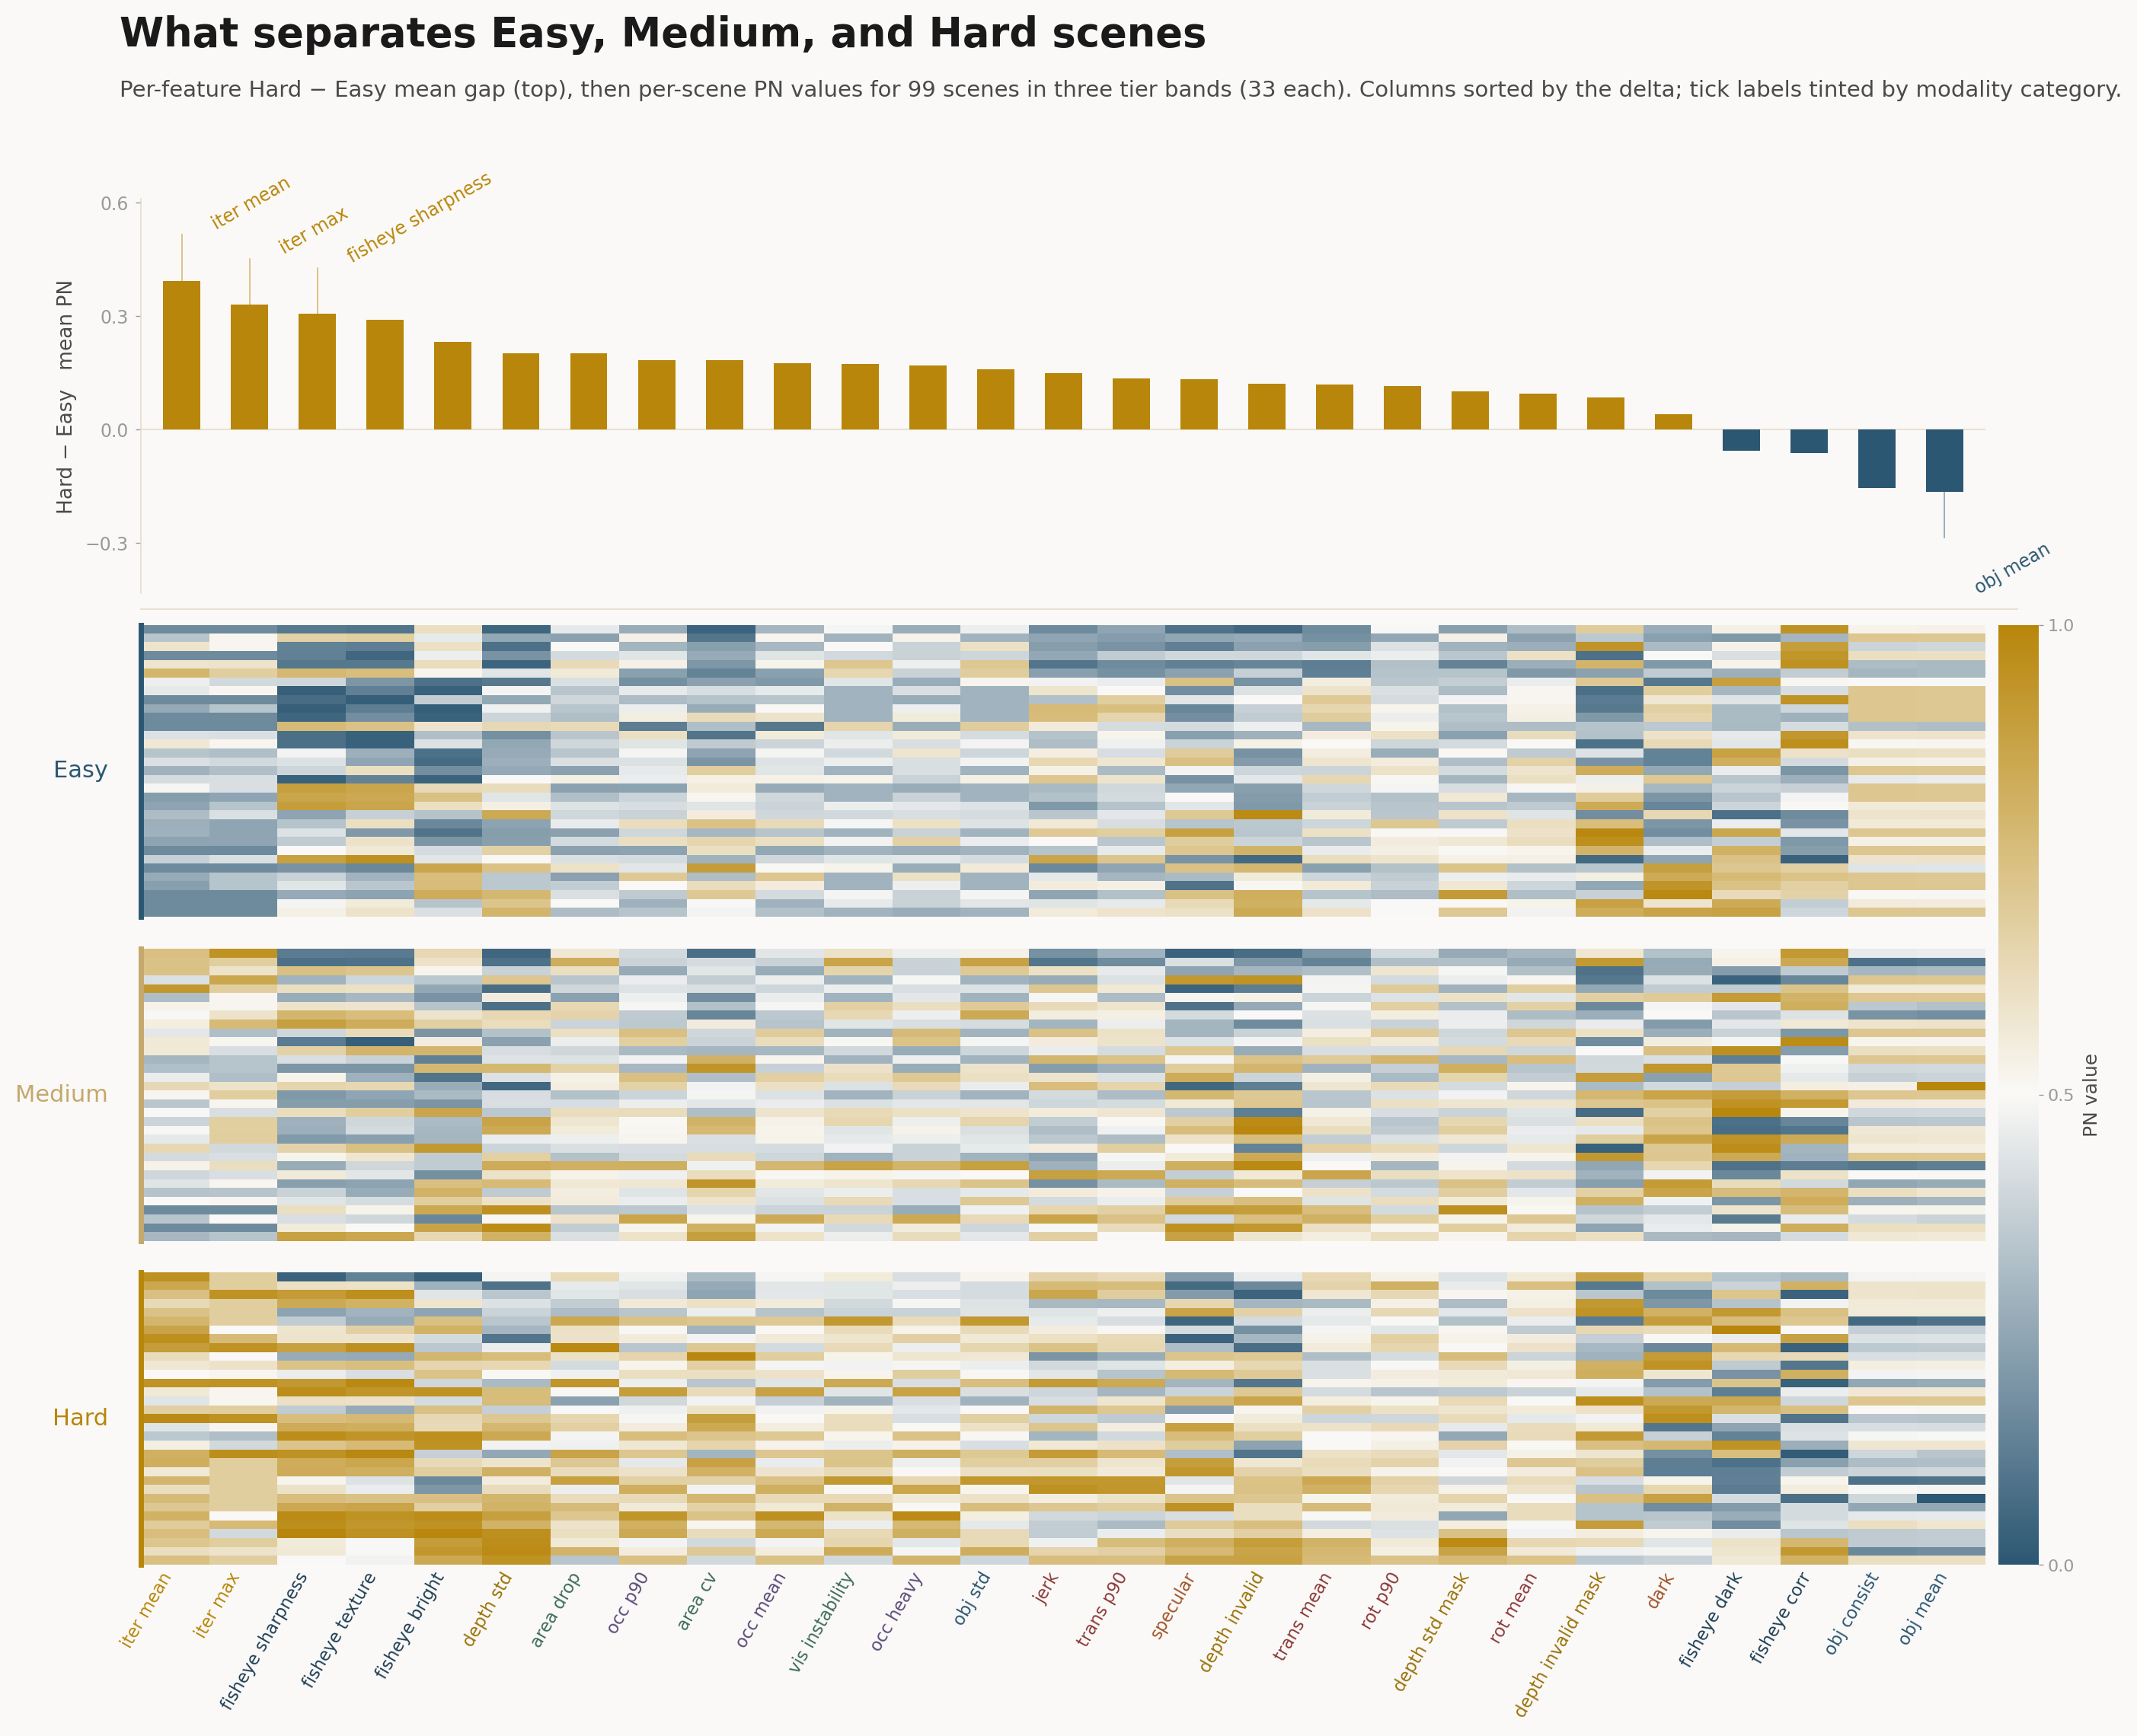
\includegraphics[width=\linewidth]{assets/images/supp_clustermap.png}
\caption{\textbf{What separates Easy, Medium, and Hard scenes.} \emph{Top:} per-feature \textsc{Hard} $-$ \textsc{Easy} mean PN gap, sorted descending. Red bars (positive gap) mark features that are systematically elevated in Hard scenes; teal bars (negative gap) mark features that lean toward Easy. The three most Hard-discriminative features are annotated inline. \emph{Bottom:} per-scene PN values for all 99 scenes, split into three horizontal bands by primary effort\_stratified\_v1 tier (33 scenes each, by tertile cut on the per-scene combined RPX-DS score). Columns are in the same order as the delta bar above; the diverging colormap is centred on the dataset median (0.5), so above-median cells render warm and below-median cells render cool. Visual reading: the Hard band runs warm on the left (where the delta is large and positive) and the Easy band runs cool there, with both bands converging toward the right where the delta crosses zero. X-axis tick labels are tinted by modality category.}
\label{fig:supp-clustermap}
\end{figure}

\begin{figure}[h]
\centering
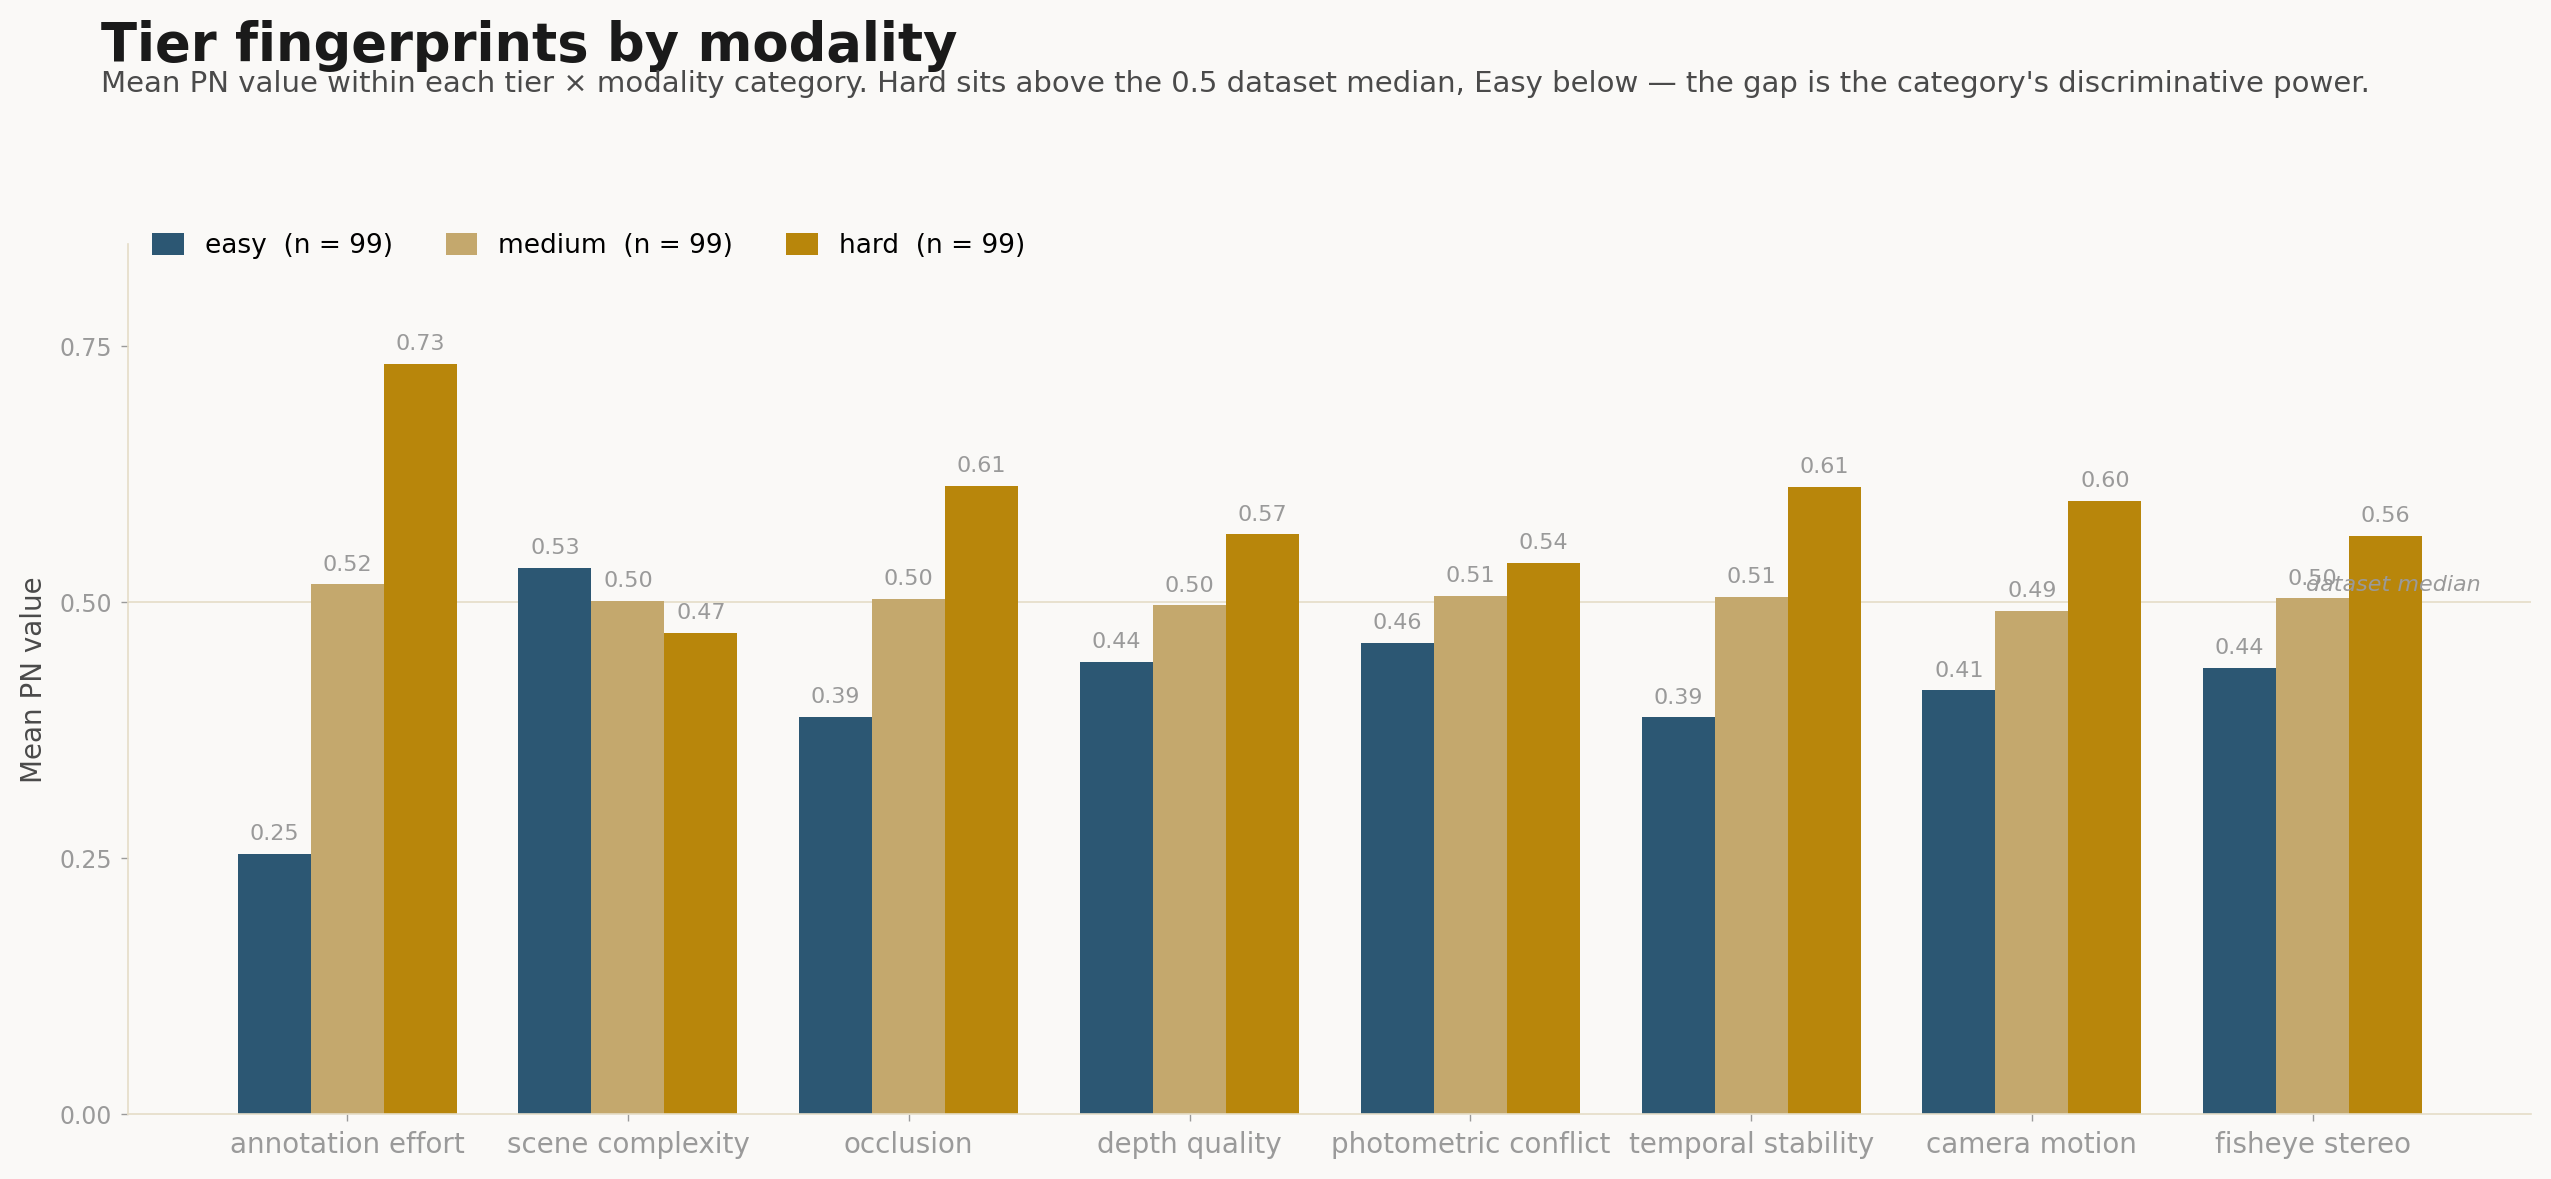
\includegraphics[width=\linewidth]{assets/images/supp_tier_fingerprint.png}
\caption{\textbf{Per-tier fingerprint --- which features pull a scene into each tier.} Mean percentile-normalised feature value within each tier, with the dataset median (0.5) marked. Easy entries (top) sit predominantly below 0.5 across most features; Hard entries (bottom) sit predominantly above 0.5. Annotation-effort features (leftmost two bars, blue) show the largest tier-to-tier swing, which is consistent with the effort-anchored weighting; perception features show the next-largest swings, with depth quality and occlusion notably elevated in the Hard tier.}
\label{fig:supp-tier-fingerprint}
\end{figure}

\begin{figure}[h]
\centering
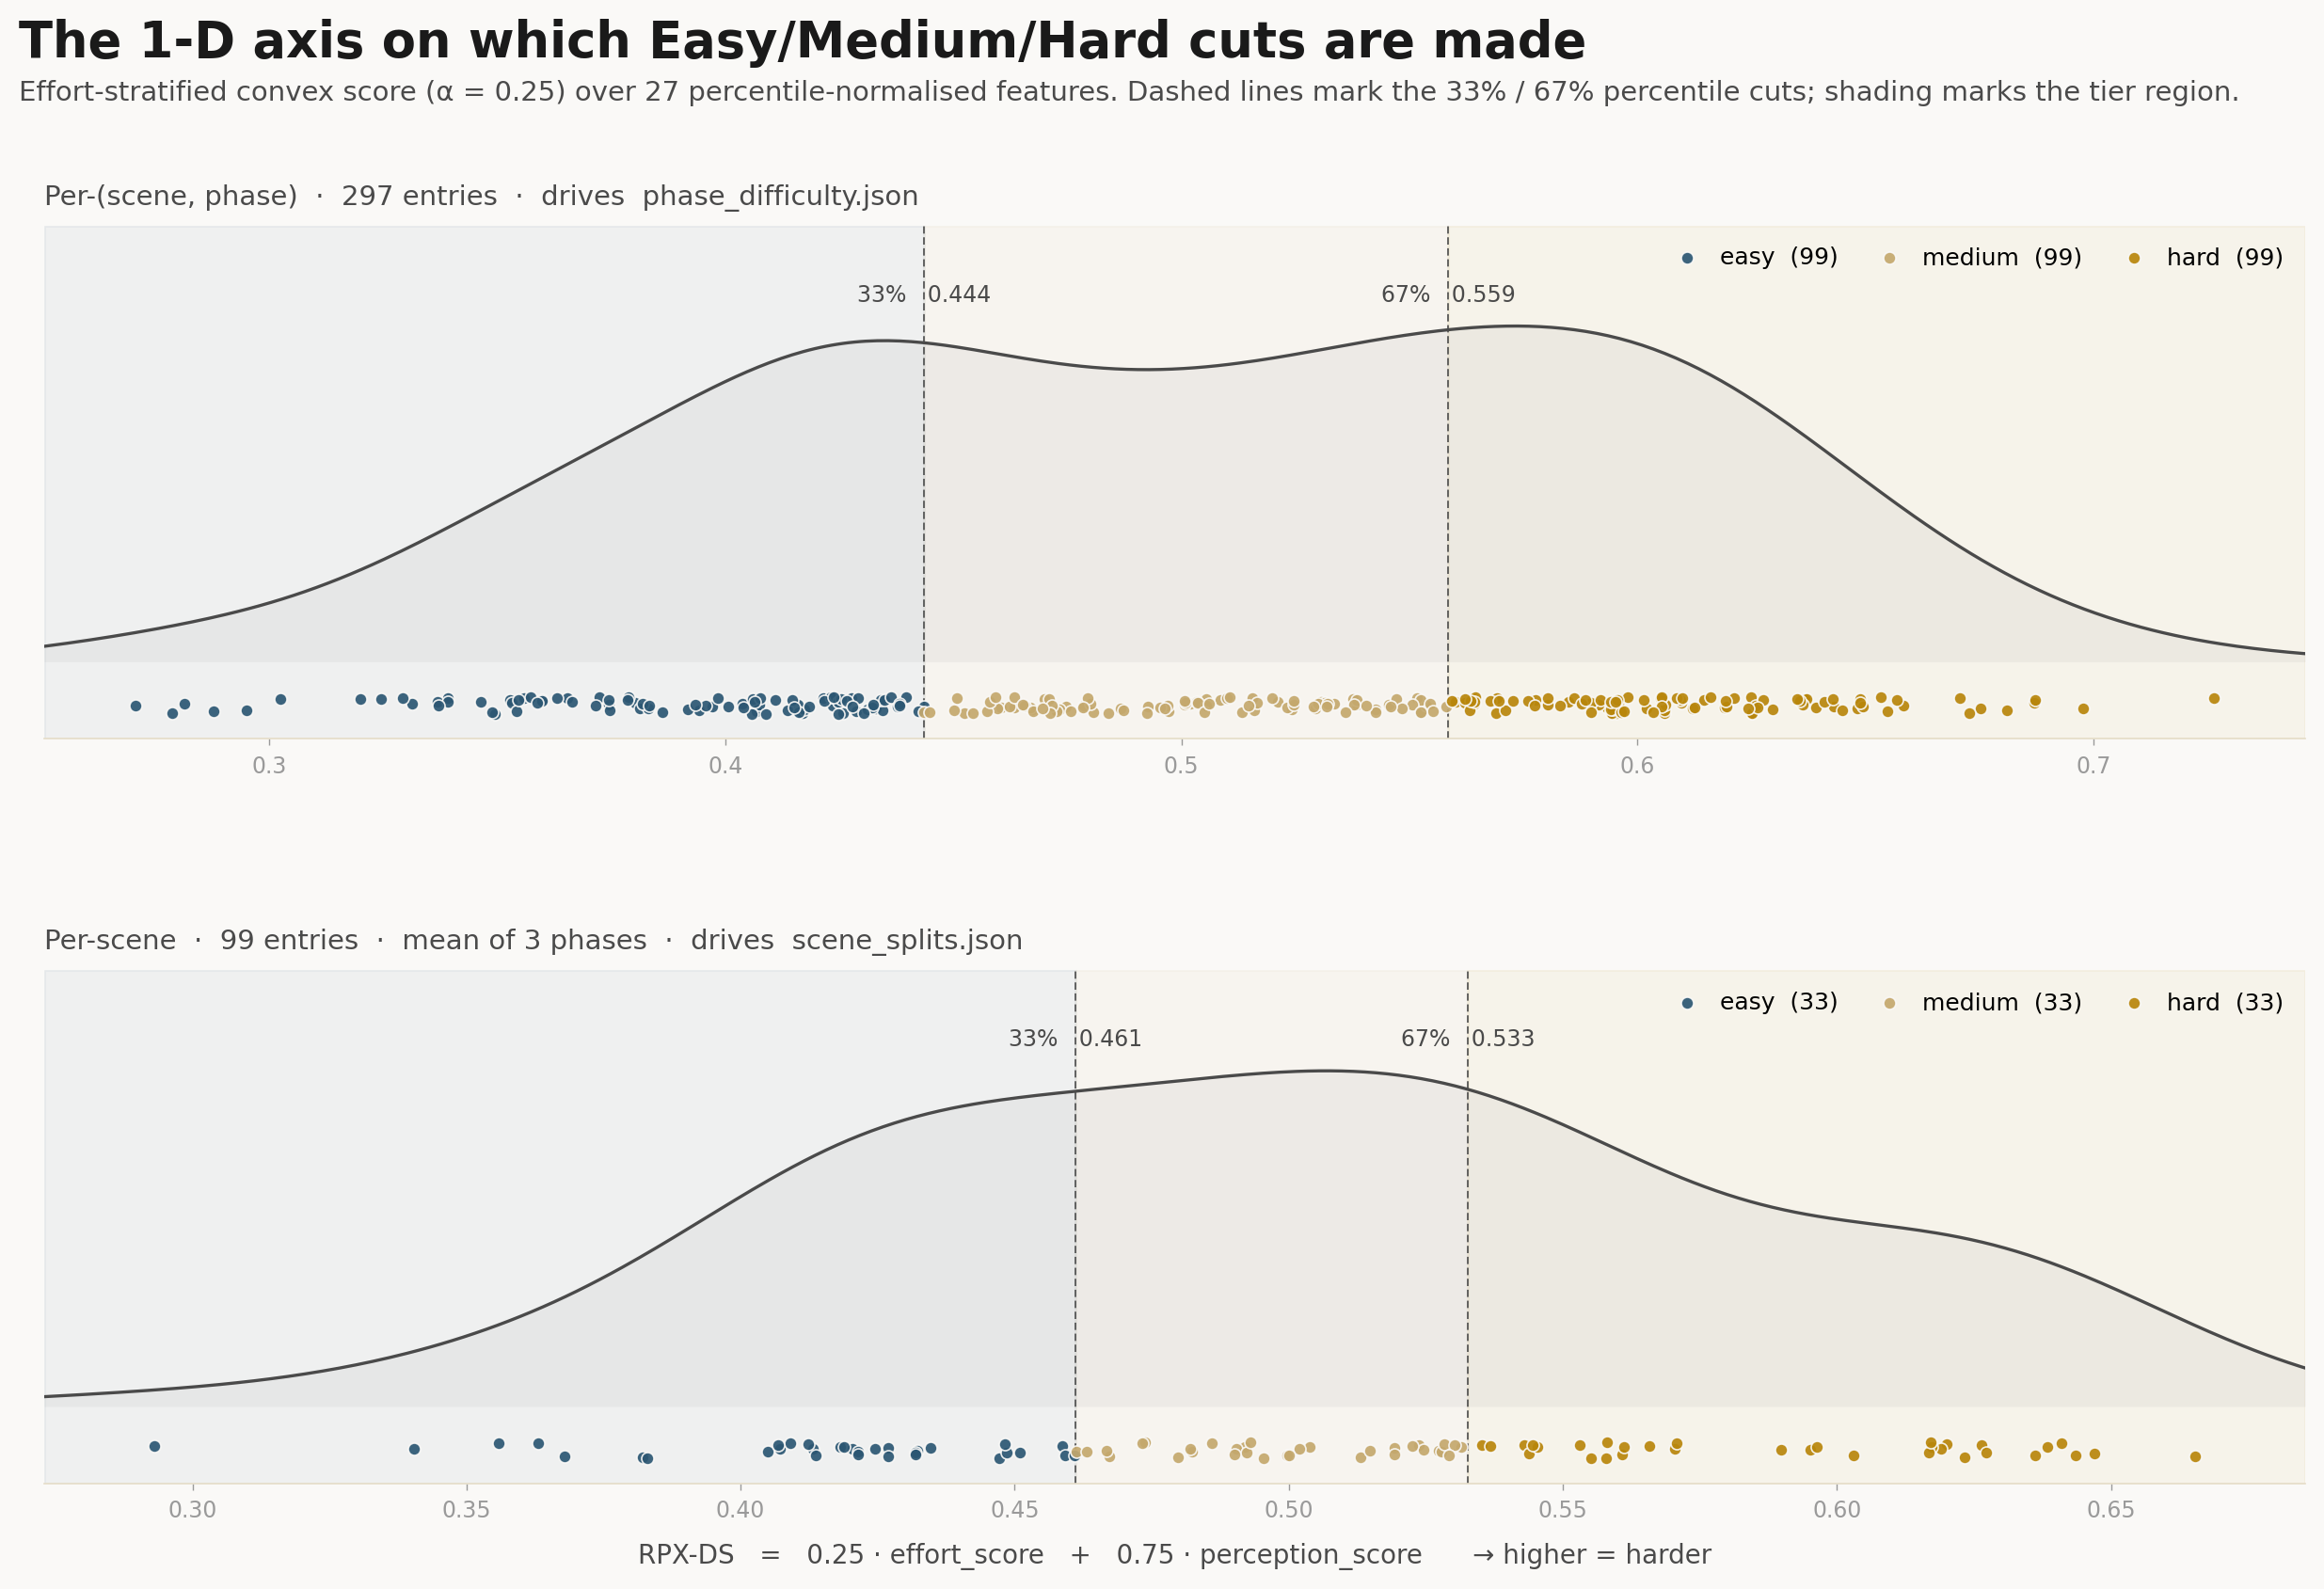
\includegraphics[width=\linewidth]{assets/images/supp_combined_score.png}
\caption{\textbf{The 1-D axis on which Easy/Medium/Hard cuts are made.} The 27-feature percentile-normalised matrix is collapsed to a single scalar via the effort-stratified convex score $\text{RPX-DS}(s,p) = 0.25 \cdot \text{effort\_score} + 0.75 \cdot \text{perception\_score}$, and the 33\% / 67\% percentile cut points (dashed lines) define the Easy / Medium / Hard boundaries. \emph{Top:} per-(scene, phase) view --- 297 entries, the level features are extracted at; tiers here drive \texttt{phase\_difficulty.json}. \emph{Bottom:} per-scene view --- 99 entries, computed as the mean of the 3 per-phase scores per scene; tiers here drive \texttt{scene\_splits.json}. Coloured dots show the assigned tier of each entry; band shading marks the tier region. The per-scene distribution is necessarily tighter than the per-phase one (averaging 3 phases shrinks variance), but the overall unimodal shape and the fact that the cuts sit on relatively gentle slopes --- rather than at sharp valleys --- is what motivates the stability tests in \S\ref{sec:appendix-esd}: small score perturbations near the cuts can flip a few entries' tier assignments without invalidating the global ordering.}
\label{fig:supp-combined-score}
\end{figure}


\section{ESD Weight Sensitivity Analysis}
\label{sec:appendix-esd}

We sample 1{,}000 weight vectors $w$ uniformly from the simplex (Dirichlet$(\mathbf{1})$) over all 27 features and recompute the RPX-DS ranking under each perturbed weight vector.
Compared to the uniform RPX-DS, the median Kendall $\tau$ between the perturbed and uniform rankings is $0.685$ (IQR: $0.630$--$0.734$), demonstrating that the relative difficulty ordering is largely preserved across scoring choices.
At the tier-assignment level, $88.6\%$ of (scene, phase) pairs retain their dominant tier (Easy/Medium/Hard) across the 1{,}000 perturbations; $11.4\%$ of pairs flip tier in fewer than 5\% of perturbations (essentially fully stable), and only $33$ of $297$ pairs ($11.1\%$) flip in more than half of perturbations.
The full per-pair stability table is shipped in the splits manifest (\texttt{benchmark/data/splits/methodology\_study/stability/weight\_perturbation.csv}).


\section{Splits Methodology Study}
\label{sec:appendix-method-study}

To validate the choice of uniform RPX-DS as the primary scoring method, we conducted a seven-layer methodology study comparing 11 scoring methods spanning every major family on the released 297 (scene, phase) feature table.
The study is fully reproducible from the dataset alone (no model results required) and is shipped as \texttt{experiments/neurips-2026/scripts/difficulty\_methodology\_study.py}.

\paragraph{Methods compared.}
\textit{Linear aggregation on percentile-normalised features:} mean (uniform\_v1, our primary), median, max, top-3 mean.
\textit{Dimensionality reduction:} first principal component (PCA-PC1).
\textit{Clustering (mapped to 3 tiers via centroid magnitude):} k-means at $k\in\{3,5,8\}$, Gaussian mixture ($k=3$, full covariance), agglomerative Ward linkage ($k=3$), and DBSCAN with $\epsilon$ chosen via the $k$-distance knee.
For visualisation, we additionally compute t-SNE, Locality Preserving Projections (LPP, \citet{he2003lpp}), and Spectral Embedding 2D projections.

\paragraph{L1: Cross-method agreement.}
Median pairwise Kendall $\tau$ between continuous scores: $0.363$.
Median pairwise Adjusted Rand Index (ARI) between categorical tiers: $0.083$.
Cross-family agreement is generally low---e.g., $\tau(\text{mean\_pn}, \text{max\_pn}) = 0.24$, $\tau(\text{mean\_pn}, \text{PCA-PC1}) = 0.39$---confirming that scoring choice is methodologically consequential and motivating the consensus-tier reporting in \S\ref{sec:features}.

\paragraph{L2: Number of clusters.}
K-means silhouette is maximised at $k=2$ (silhouette $= 0.293$); GMM silhouette is maximised at $k=3$ ($0.238$). Tibshirani's gap statistic also recommends $k=2$ (Fig.~\ref{fig:methstudy-nclusters}).
The data therefore does \textit{not} natively support a 3-cluster structure; the 33/33/34 tertile is adopted as a reporting convention because Easy/Medium/Hard is canonical in benchmarks.

\begin{figure}[h]
\centering
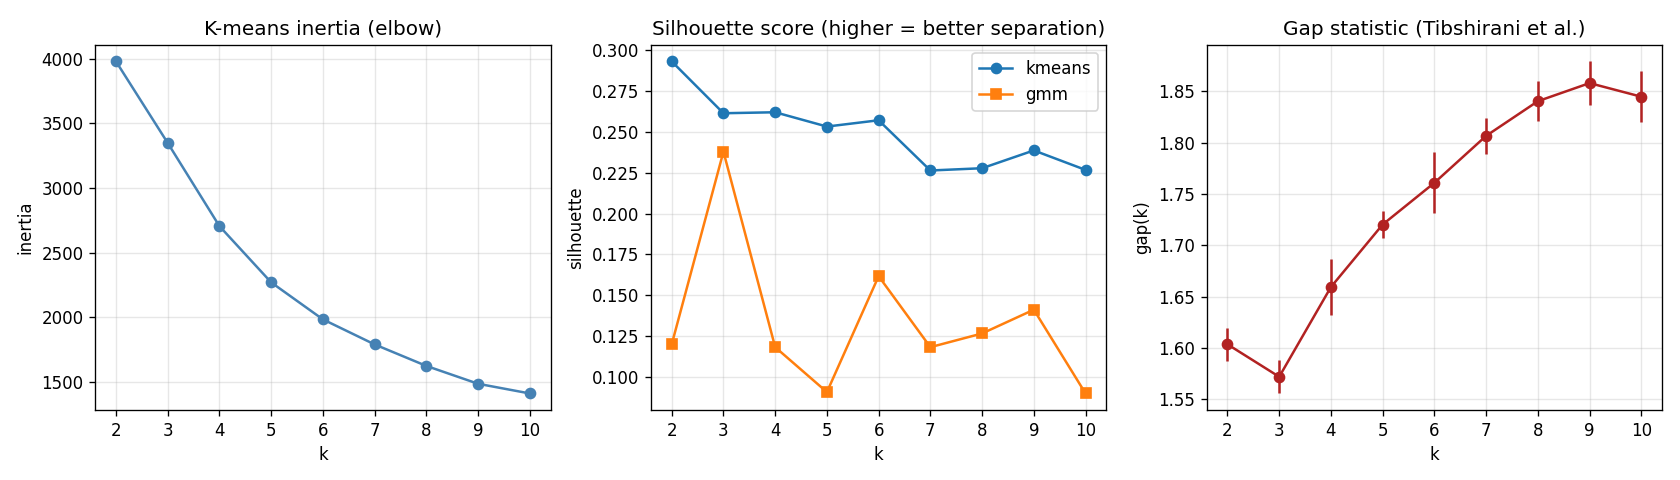
\includegraphics[width=\linewidth]{assets/images/methstudy_n_clusters_diagnostics.png}
\caption{\textbf{Cluster-count diagnostics on the 297-pair, 27-feature matrix.} K-means inertia (left) shows no sharp elbow. K-means silhouette (centre, blue) peaks at $k=2$; GMM silhouette (centre, orange) peaks at $k=3$. Tibshirani's gap statistic (right) is monotonically increasing through $k=10$; the smallest $k$ satisfying gap$(k) \geq$ gap$(k+1) - s_{k+1}$ is $k=2$. The data does not natively prefer $k=3$ — the tertile is a reporting convention.}
\label{fig:methstudy-nclusters}
\end{figure}

\paragraph{L3: Stability under perturbations.}
Three independent perturbation studies on uniform\_v1 (1{,}000 iterations each unless noted):
\textit{(a) Bootstrap subsampling (80\%):} median per-pair dominant-tier stability $= 1.000$; $89.9\%$ of pairs have $>$95\% stability across resamples; $81.1\%$ of pairs are perfectly stable.
\textit{(b) Weight perturbation (Dirichlet$(\mathbf{1})$):} median tier-flip rate $0.348$; $88.6\%$ of pairs retain dominant tier (see \S\ref{sec:appendix-esd} for the full Kendall-$\tau$ analysis).
\textit{(c) Feature dropout (drop 1/3 random features, 200 iterations):} median tier-flip rate $0.275$; $23.9\%$ of pairs flip in $<$5\% of dropouts.
The full per-pair distributions are in Fig.~\ref{fig:methstudy-stability}.

\begin{figure}[h]
\centering
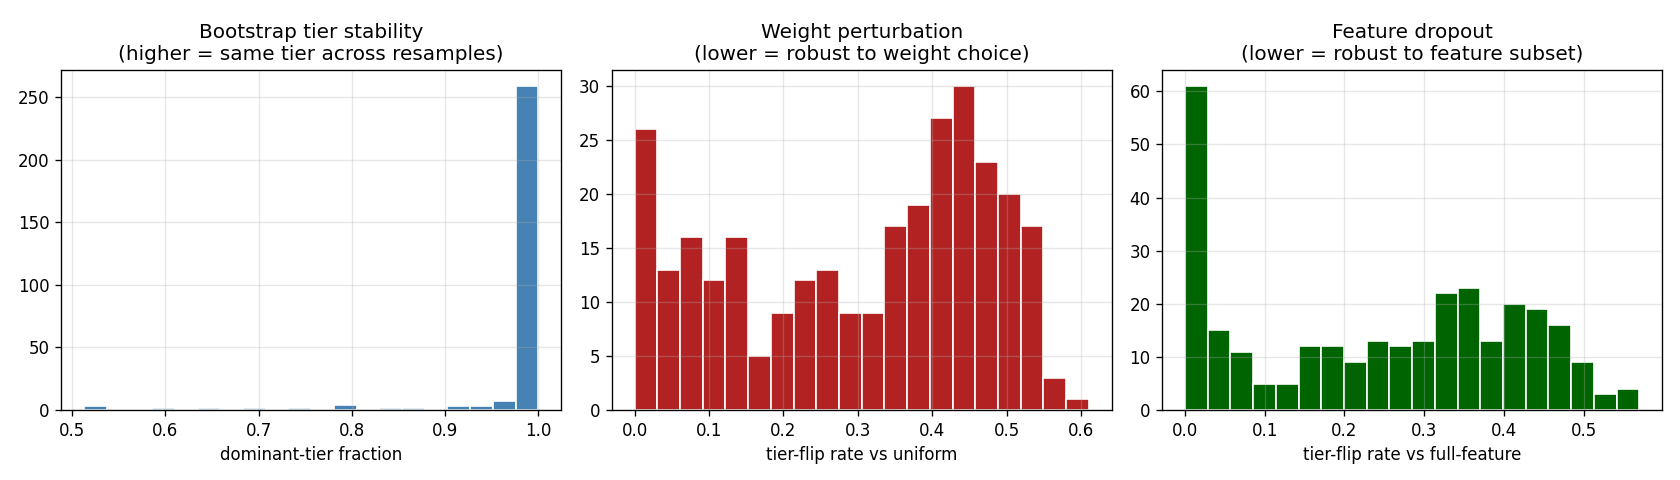
\includegraphics[width=\linewidth]{assets/images/methstudy_stability_distribution.png}
\caption{\textbf{Stability of the uniform\_v1 tier assignment under three perturbation studies.} Bootstrap subsampling (left, blue) is dominated by the mass at 1.0 — the assignment is essentially invariant to which 80\% of scenes is sampled. Weight perturbation (centre, red) is bimodal: a stable subpopulation flips little and a sensitive subpopulation flips ${\sim}50\%$ of the time. Feature dropout (right, green) shows a stable mode at 0 and a long tail. Bootstrap-rock-stable but weight-sensitive — the case for shipping the consensus tier alongside any single primary method.}
\label{fig:methstudy-stability}
\end{figure}

\paragraph{L4: Outliers.}
Twelve (scene, phase) pairs exceed the $\chi^2_{27}(0.99)$ Mahalanobis-distance threshold in the percentile-normalised feature space. The top entries by distance are \texttt{scene100.jsom.atrium} interaction phase ($d=11.95$), \texttt{scene18.su.CHECKERBOARD} clutter phase ($d=10.86$), and \texttt{scene74.ecsw.atriumStairs} clean phase ($d=7.69$). Two of these (\texttt{scene100} and \texttt{scene74}) coincide with documented T265 tracking-failure events during capture, demonstrating that the methodology surfaces genuine data quality issues from the feature distribution alone.

\paragraph{L5: Cross-method consensus.}
Across the 11 methods (DBSCAN excluded as degenerate---it found no density modes in the 27D feature space), only $24$ of $297$ pairs ($8.1\%$) receive unanimous tier assignment. $104$ pairs ($35.0\%$) are split between two tiers, and $169$ pairs ($56.9\%$) span all three (Fig.~\ref{fig:methstudy-consensus}).
The consensus tier (majority vote) is shipped alongside uniform\_v1 in the splits manifest.

\begin{figure}[h]
\centering
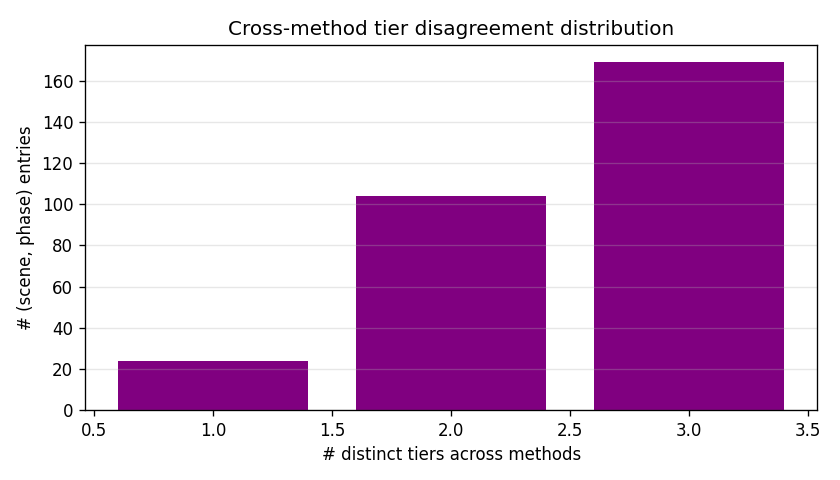
\includegraphics[width=0.55\linewidth]{assets/images/methstudy_consensus_disagreement.png}
\caption{\textbf{Cross-method tier disagreement.} Histogram of distinct tiers assigned per (scene, phase) across 11 scoring methods. Only 8.1\% of pairs receive unanimous agreement; the majority span 2 or 3 tiers. The consensus tier (majority vote) is shipped alongside the primary uniform\_v1 tier.}
\label{fig:methstudy-consensus}
\end{figure}

\paragraph{L6: Phase signature.}
The maximum ARI between any clustering method's labels and the capture-phase index (clutter/interaction/clean) is $0.182$ (k-means at $k=8$); for $k=3$ partitions specifically: k-means $0.177$, GMM $0.036$, Ward $0.003$, DBSCAN $0.003$. Feature space therefore captures perception difficulty rather than capture-protocol identity---validating that ESD splits are a difficulty stratification, not a phase classifier.

\paragraph{Per-feature contribution by tier.}
Fig.~\ref{fig:methstudy-features} shows the mean percentile-normalised value of each feature within each Easy/Medium/Hard tier. Hard scenes are higher than Easy on most features---confirming the score is broadly difficulty-tracking rather than driven by a single modality. Three features show inverted ordering: $f_{\text{obj-mean}}$ and $f_{\text{obj-consist}}$ (densely-arranged static scenes are ``Easy'' in the multi-feature sense), and $f_{\text{fisheye-corr}}$ (transparent or motion-blurred scenes break stereo correlation, marking them as Hard with low corr).

\begin{figure}[h]
\centering
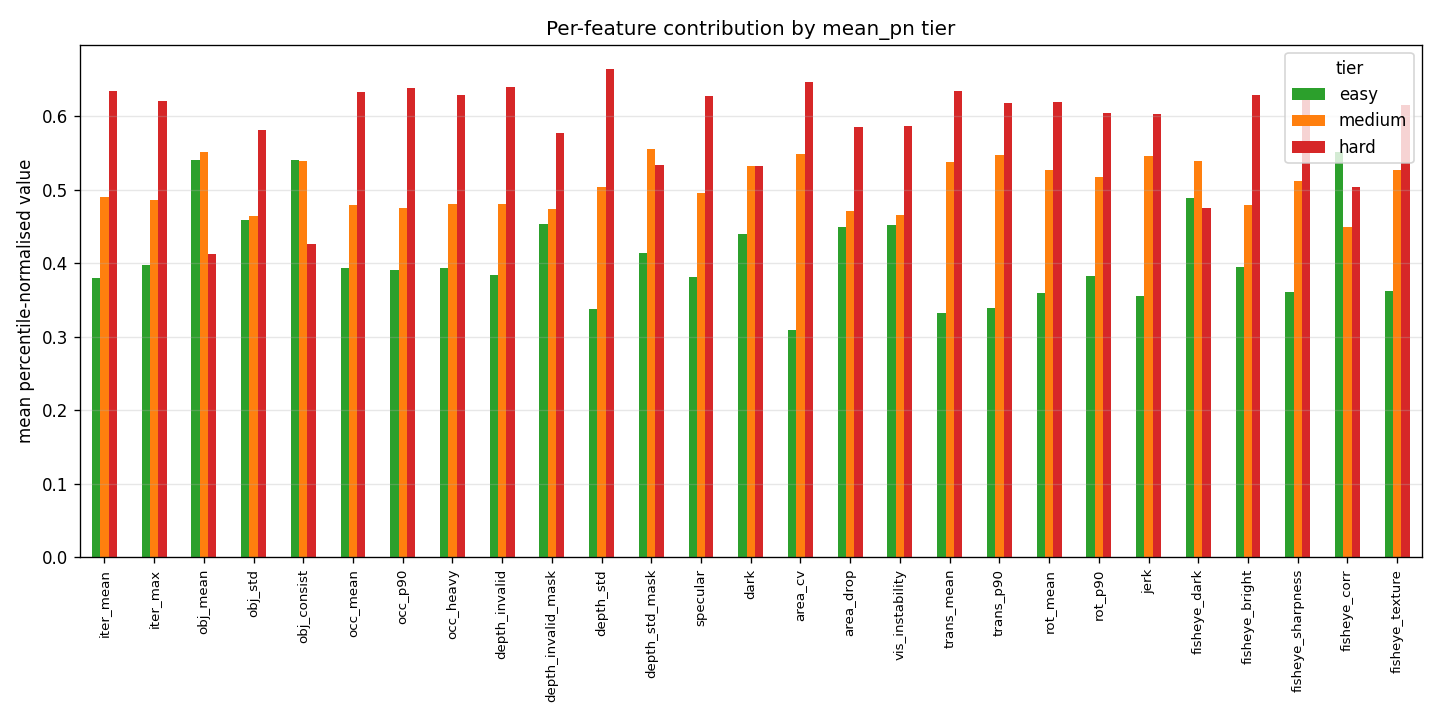
\includegraphics[width=\linewidth]{assets/images/methstudy_feature_contributions_by_tier.png}
\caption{\textbf{Per-feature mean percentile-normalised value by uniform\_v1 tier.} Hard tier (red) is uniformly higher than Easy (green) on most features, confirming the multi-modal nature of the difficulty signal. Three inversions ($f_{\text{obj-mean}}$, $f_{\text{obj-consist}}$, $f_{\text{fisheye-corr}}$) reveal that scene complexity ${\neq}$ scene difficulty: densely arranged but well-lit static scenes can still be Easy, while sparsely arranged but transparent or moving scenes are Hard.}
\label{fig:methstudy-features}
\end{figure}

\paragraph{Reproducibility.}
All numbers above are deterministic given seed=0; the full study (tables, plots, and per-entry assignments under all 11 methods) ships under \texttt{benchmark/data/splits/methodology\_study/}, with input file SHA-256 stamped into \texttt{provenance.json}.


\section{Ground-Truth Annotation Pipeline}
\label{sec:appendix-annotation}

This section documents the three major annotation pipelines in detail.
Figure~\ref{fig:mask-pipeline} illustrates the mask annotation workflow,
Figure~\ref{fig:qa-generation} illustrates the QA ground-truth generation,
and Figure~\ref{fig:pose-refinement} illustrates the camera pose refinement procedure.

\subsection{Instance Mask Annotation}
\label{sec:appendix-masks}

\begin{figure}[h]
    \centering
    % \includegraphics[width=\linewidth]{assets/images/mask-pipeline.pdf}
    \todo{Figure: mask annotation pipeline diagram — SAM2 auto $\to$ GroundingDINO bbox proposals $\to$ human iterative refinement UI $\to$ final masks. Show example frames at each stage.}
    \caption{Instance mask annotation pipeline. (1)~SAM2 auto-mode generates initial masks.
    (2)~GroundingDINO proposes bounding boxes for missed objects using text prompts from the object questionnaire.
    (3)~A human annotator iteratively refines boundaries in a custom UI until sub-pixel accuracy at object edges.
    The refinement iteration count $k_j$ per instance feeds ESD (\S\ref{sec:features}).}
    \label{fig:mask-pipeline}
\end{figure}

SAM2~\citep{ravi2024sam2} in automatic mode generates initial instance masks for each keyframe.
GroundingDINO~\citep{liu2024groundingDINO} provides complementary bounding-box proposals using per-object category names from the FewSOL questionnaire, catching objects that SAM2's class-agnostic mode misses (e.g.\ transparent items, thin utensils).
A custom annotation interface then enables iterative human refinement: annotators adjust mask boundaries, split merged instances, and add missing objects until edges align with object contours at sub-pixel accuracy.
The refinement iteration count $k_j$ per instance is recorded and directly feeds the ESD difficulty model (Section~\ref{sec:features})---scenes requiring more human correction are empirically harder for models.

\paragraph{Tracklets.}
SAM2 video propagation with human-corrected keyframe initialisation produces dense tracklets with consistent IDs across each phase.
Annotators verify ID consistency at phase boundaries and correct drift or ID switches introduced by fast hand motion during interaction.

\subsection{QA Ground-Truth Generation}
\label{sec:appendix-qa}

\begin{figure}[h]
    \centering
    % \includegraphics[width=\linewidth]{assets/images/qa-generation.pdf}
    \todo{Figure: QA generation pipeline — (a) human-authored template bank with robotics-grounded question types, (b) per-frame instantiation using visibility masks + bbox geometry + questionnaire attributes, (c) example Q/A pairs showing phase-varying answers.}
    \caption{QA ground-truth generation. Humans author question templates grounded in robotics operator needs (left).
    Templates are instantiated deterministically per frame using object visibility masks, bounding-box geometry, and questionnaire attributes (centre).
    The same question produces different correct answers across phases (right).}
    \label{fig:qa-generation}
\end{figure}

\paragraph{Template design.}
A set of question templates was authored by hand to reflect the information needs of a robot operator or planner.
Templates fall into four categories:
\textbf{(i)~Identity}: ``What objects are on the table?'', ``Is there a \{category\}?'';
\textbf{(ii)~Attribute verification}: ``What colour is the \{object\}?'', ``What material is the \{object\}?'';
\textbf{(iii)~Counting}: ``How many objects are visible?'';
\textbf{(iv)~Spatial relations} (D5): ``What is to the left/right/above/below of the \{object\}?''.
All templates use crowd-sourced natural-language object descriptions from FewSOL questionnaires~\citep{padalunkal2023fewsol} (\S\ref{sec:dataset}), matching how real users command robots.

\paragraph{Instantiation.}
For each frame $t$, templates are instantiated deterministically:
(a)~per-frame visibility is determined from instance masks (an object is ``visible'' if its mask area exceeds a minimum threshold);
(b)~identity and attribute answers are read from the questionnaire;
(c)~spatial relations are computed in the \textit{image plane} using polar coordinates centred on the reference object's bounding-box centroid.
This yields \todo{X} Q/A pairs per scene across all phases.
Critically, the same question has \textit{different correct answers} across phases (e.g.\ objects are rearranged, new objects become visible), making this, to our knowledge, the first perception QA benchmark with phase-varying ground truth.

\paragraph{Spatial relation definition.}
All spatial relations are defined in the image plane: ``left'' = centroid with smaller $x$-coordinate; ``above'' = smaller $y$-coordinate; ``near'' = Euclidean distance $<\tau_\text{near}$ pixels.
This matches how VLMs process images and avoids ambiguity from world-frame perspective.

\subsection{Camera Pose Refinement}
\label{sec:appendix-pose}

\begin{figure}[h]
    \centering
    % \includegraphics[width=\linewidth]{assets/images/pose-refinement.pdf}
    \todo{Figure: pose refinement pipeline — T265 raw VIO trajectory $\to$ outlier rejection $\to$ optional loop closure $\to$ refined trajectory. Show before/after trajectory overlay on a sample scene.}
    \caption{Camera pose refinement. Raw T265 VIO at 200\,Hz is downsampled to 30\,fps,
    filtered for outlier jumps, and validated via loop-closure analysis on closed-loop sequences.}
    \label{fig:pose-refinement}
\end{figure}

T265 VIO provides 6-DoF camera pose at 200\,Hz, downsampled to 30\,fps to align with D435 frames.
Raw T265 odometry is used as the pose reference---no offline bundle adjustment is applied, preserving the noise profile that deployed robots would encounter with the same sensor.
Over ${\sim}$250 frames (${\sim}$8\,s per phase), drift is bounded to $<$\todo{X}\,cm / $<$\todo{X}$^\circ$ via loop-closure analysis on \todo{N} closed-loop sequences where the camera returns to its starting position.
Outlier frames with $\Delta t > \todo{X}$\,cm or $\Delta R > \todo{X}^\circ$ between consecutive frames are flagged and excluded from temporal stability (TS) computation.

\paragraph{Depth ground truth.}
Raw D435 structured-light depth; invalid pixels (specular reflection, transparency, range limits) are flagged and excluded from evaluation.
No inpainting is applied---models are evaluated only on pixels where the sensor produces valid returns.

\paragraph{Language annotations.}
Per-object attributes (category, colour, material, shape) from FewSOL~\citep{padalunkal2023fewsol} questionnaires serve as referring expressions for grounding evaluation and as the vocabulary source for QA template instantiation (\S\ref{sec:appendix-qa}).


\section{Per-Task Detailed Results}
\label{sec:appendix-per-task}

% ── TODO(results): one table per task with full breakdowns ──
\todo{One table per task (D1--D5) with:
All models (including appendix-only: DA-V2 Base, Prompt DA, MiDaS, SAM2 Small, DITO, RO-ViT, etc.).
Per-ESD columns (Easy / Medium / Hard).
Per-phase columns ($\mathcal{P}_{\text{clu}}$ / $\mathcal{P}_{\text{int}}$ / $\mathcal{P}_{\text{cln}}$).
Full metric suite (not just primary metric).
Params, FLOPs, median latency.}


\section{Camera Motion Statistics}
\label{sec:appendix-motion}

% ── TODO(data): compute from T265 poses ──
\todo{Full-page figure:
(a) Histogram of $\Delta t$ (cm/frame) across 100 scenes $\times$ 3 phases.
(b) Histogram of $\Delta R$ (deg/frame).
(c) Histogram of jerk.
(d) Overlay with published platform motion profiles from Stretch RE2, Unitree H1, Fetch, Spot.}


\section{Dataset Object Taxonomy}
\label{sec:appendix-objects}

% ── TODO(data): compile from annotation metadata ──
\todo{Full object taxonomy:
$\sim$70 categories with supercategory assignments, instance counts, YCB/FewSOL overlap markers.
Example images.}


\section{Text vs.\ Visual Prompting: Extended Analysis}
\label{sec:appendix-prompting}

% ── TODO(results): extended D3 analysis ──
\todo{Extended comparison of text-prompted (GroundingDINO, OWL-ViT, YOLO-World, Qwen2-VL)
vs.\ image-prompted (DE-ViT, NIDS-Net, Qwen2-VL with visual prompt) detection.
Per-ESD, per-phase breakdown.
Analysis of which object categories benefit most from each prompting mode.
Failure case examples: text prompt fails when spatial relations change; visual prompt fails under viewpoint shift.}


\section{\coolname{} Toolkit: Extended Documentation}
\label{sec:appendix-toolkit}

This appendix provides extended documentation for the \texttt{rpx-benchmark} toolkit described in Section~\ref{sec:toolkit}.

\paragraph{Python API usage example.}
\begin{verbatim}
from rpx_benchmark import (
    RPXDataset, BenchmarkRunner,
    MetricSuite, TaskType
)

dataset = RPXDataset.from_manifest("rpx_test.json")
model   = MyDepthModel()  # subclasses BenchmarkModel
suite   = MetricSuite.for_task(TaskType.MONOCULAR_DEPTH)
runner  = BenchmarkRunner(model, dataset, suite)

result, dr = runner.run_with_deployment_readiness(
    primary_metric="abs_rel",
    model_name="MyDepthModel"
)
print(dr.summary())
\end{verbatim}

The \texttt{dr.summary()} output:
\begin{verbatim}
--- RPX Deployment Readiness: MyDepthModel ---
  S_overall  = 0.134 (AbsRel, lower=better)
  STR_{C->I} = -0.023 (interaction drop)
  STR_{I->L} = +0.018 (recovery)
  TS         = 0.891 (temporal stability)
  SGC        = 0.672 (geometric coherence)
  Params     = 335M   FLOPs = 211G
  Latency    = 45ms (median, per frame)
\end{verbatim}

\paragraph{Adding a new task.}
\begin{verbatim}
from rpx_benchmark.tasks import register_task, TaskSpec
register_task(TaskSpec(
    name="affordance_prediction",
    runner=my_affordance_runner,
    metrics=["auc", "f1"],
    input_modalities=["rgb", "depth"],
))
\end{verbatim}

\paragraph{Adding a new metric.}
\begin{verbatim}
from rpx_benchmark.metrics import BaseMetric, register_metric
class GraspAlignment(BaseMetric):
    def compute(self, pred_mask, gt_depth):
        return score
register_metric("grasp_alignment", GraspAlignment)
\end{verbatim}

\paragraph{CI.} 138 offline tests, Python 3.10/3.11/3.12, GitHub Actions, zero network deps.
MkDocs + mkdocstrings auto-docs. Ruff lint.


\section{Cross-Task Ranking Agreement}
\label{sec:appendix-cross-task}

% ── TODO(analysis): cross-task correlation ──
\todo{(a) Kendall $\tau$ of $S_\text{overall}$ rankings for task pairs sharing $\geq$2 models.
(b) Kendall $\tau$ of scene difficulty rankings across tasks (ESD consistency).
(c) For shared-backbone models: does deployment readiness transfer across tasks?}


\section{Croissant Metadata and Datasheet}
\label{sec:appendix-croissant}

\coolname{} is documented using Croissant~\citep{akhtar2024croissant} with core and RAI fields, as required by NeurIPS 2026 E\&D Track.
\textbf{Core:} name, URL, licence (CC BY 4.0), format, record sets for each modality.
\textbf{RAI:} collection protocol, consent, PII assessment (none), annotation methodology, known biases (indoor-dominant, D435 range, human motion profile).
The Croissant JSON is included with the supplementary materials and hosted on HuggingFace.

\section{Scope, Assumptions, and Output-vs-Feature Evaluation}
\label{sec:appendix-scope}

\coolname{} is designed to test the claim: \textit{pretrained perception backbones differ in deployment robustness, and this difference is not predictable from standard accuracy alone.}

\paragraph{Output-level vs.\ feature-level evaluation.}
Robot learning systems consume perception at two levels.
\textbf{(a)~As raw signals:} modular systems (OK-Robot, DP3, AnyGrasp~\citep{liu2024okrobot, ze2024dp3}) directly consume depth maps, bounding boxes, and masks---for these, \coolname{} evaluates the signal the robot directly consumes.
\textbf{(b)~As encoded features:} VLAs ($\pi_0$, OpenVLA, GR00T) consume frozen or fine-tuned encoder activations, never producing an explicit depth map or detection.
For these, \coolname{}'s task-level metrics serve as \textit{proxies} for feature quality: a backbone whose outputs exhibit low temporal stability (TS) or poor phase-transition robustness (STR) has representations that fail to stably encode scene geometry or handle occlusion, and an action-conditioned decoder is unlikely to fully recover information the encoder failed to capture.
Furthermore, \coolname{}'s VLM evaluation (D4/D5) directly tests the same VLMs (PaliGemma, Qwen2-VL) that VLAs are built on.
The downstream validation in \S\ref{sec:downstream} empirically tests whether \coolname{}'s rankings transfer to task-level success.

\paragraph{Additional assumptions.}
(i)~Human-carried capture is a valid motion proxy (validated in \S\ref{sec:dataset} and Appendix~\ref{sec:appendix-motion}).
(ii)~100 scenes are representative of deployment environments.
(iii)~Zero-shot evaluation reflects deployment conditions.

\paragraph{Out of scope.}
Navigation-specific perception, sensing outside the D435/T265 envelope (0.3--3\,m indoor + matched outdoor), and platforms with non-humanoid kinematics (e.g., fixed-base arms with restricted viewpoints).

